\section{Git Introduction}

\begin{frame}[fragile]{Installing git}

    \textbf{Debian:}
    \begin{lstlisting}
    apt install git
    \end{lstlisting}

    \textbf{Arch Linux:}
    \begin{lstlisting}
    pacman -S git
    \end{lstlisting}

    \textbf{Fedora:}
    \begin{lstlisting}
    yum install git
    \end{lstlisting}

    \begin{description}
        \item{For Linux:} \url{http://git-scm.com/download/linux}
        \item{For Mac:} \url{http://git-scm.com/download/mac}
        \item{For Windows:} \url{http://git-scm.com/download/win}
    \end{description}

\end{frame}

\begin{frame}[fragile]{How it NOT works}
    \begin{figure}
        \centering
        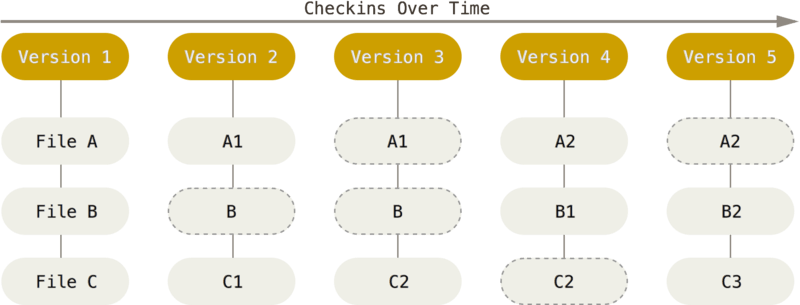
\includegraphics[width=0.8\textwidth]{img/snapshotbased.png}
        \caption{storing snapshots over time}
    \end{figure}
\end{frame}

\begin{frame}[fragile]{How it works}
    \begin{figure}
        \centering
        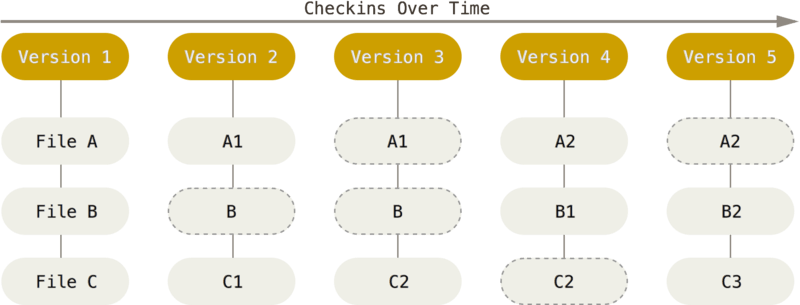
\includegraphics[width=0.8\textwidth]{img/snapshotbased.png}
        \caption{storing snapshots over time}
    \end{figure}
\end{frame}
%\begin{frame}{How it works}

    %\begin{itemize}
        %\item most operations are local
        %\item entire history is locally available
    %\end{itemize}

    %integrety
    %everything is check-summed before and then referrenced to by that checksum
    %sha1 40 charcter string hex decode
    %git stores everything by hash value of its contents instead of its filename

    %git only adds data

    %three states
    %- commited
    %- modified
    %- staged
    %- (untracked)

%\end{frame}

\begin{frame}{What is a git repository?}

    \begin{figure}
        \centering
        \includegraphics[width=0.9\textwidth]{img/three_states.png}
    \end{figure}
\end{frame}

\begin{frame}{Basic Workflow}
    \begin{enumerate}
        \item Modify files in your working directory.
        \item Stage the files, adding snapshots of them to your staging area.
        \item Commit, stores the snapshot in the staging area permanently in
            your git directory.
        \item Push your commits to an remote repository on a server.
    \end{enumerate}
\end{frame}

\defverbatim\setusername{%
    \scriptsize
    \verb+git config --global user.name "Max Mustermann"+
    \newline
}
\defverbatim\setusermail{%
    \scriptsize
    \verb+git config --global user.mail "max.mustermann@example.org"+
    \newline
}

\begin{frame}{Configure Git}

    \emph{Place where the git configuration can live:}
    \vspace{1cm}

    % TODO: take a table for that
    \begin{itemize}
            \item \textbf{/etc/gitconfig} system wide configuration
                \textit{-\,-system}
            \item \textbf{~/.gitconfig} or \textbf{~/.config/gitconfig}  user wide configuration \textit{-\,-global}
            \item \textbf{.git/config} repository specific configuration
    \end{itemize}

\end{frame}

\begin{frame}[fragile]{Configure Git}
    \textbf{Show your configuration:}
    \begin{lstlisting}
        git config --list
    \end{lstlisting}
    \textbf{Show specific configuration value:}
    \begin{lstlisting}
        git config user.name
    \end{lstlisting}
    \textbf{Define an alias:}
    \begin{lstlisting}
        git config alias.st=git status
    \end{lstlisting}
    \textbf{Enable highlighting:}
    \begin{lstlisting}
        git config --global color.ui=always
    \end{lstlisting}
\end{frame}

\begin{frame}[fragile]{Setup Your Environment}
    \emph{Three essentail configuration values you should have set.}
    \vspace{1cm}

    \textbf{Your name:}
    \begin{lstlisting}
        git config --global user.name "Max Mustermann"
    \end{lstlisting}
    \textbf{Your email address:}
    \begin{lstlisting}
        git config --global user.mail "max@example.org"
    \end{lstlisting}
    \textbf{Your editor:}
    \begin{lstlisting}
        git config --global core.editor "vim"
    \end{lstlisting}
\end{frame}

\begin{frame}[fragile]{Lets Start\ldots}
    \textbf{Start from scratch:}
    \begin{lstlisting}
mkdir my_new_project
cd my_new_project
git init
    \end{lstlisting}
    \textbf{Get a local copy of a repository that already exist.}
    \begin{lstlisting}
git clone https://github.com/blastmaster/ta-git_intro.git
git clone -b <branchname> <GIT_URL>
    \end{lstlisting}
\end{frame}

\begin{frame}[fragile]{Follow the changes}
    \textbf{What is the status of your local repo?}
    \begin{lstlisting}
        git status
    \end{lstlisting}
    \textbf{What happens so far?}
    \begin{lstlisting}
        git log
    \end{lstlisting}
    \textbf{What has changed?}
    \begin{lstlisting}
        git diff [--staged]
    \end{lstlisting}
    \textbf{Who has changed?}
    \begin{lstlisting}
        git blame
    \end{lstlisting}
\end{frame}

\begin{frame}[fragile]{Ignoring Files}
    \emph{Ignore files that follow a specific pattern with a \textbf{.gitignore} file}

    \textit{.gitignore} rules:
    \begin{itemize}
        \item Black lines or lines starting with \# are ignored.
        \item Standard glob pattern work.
        \item You can start patterns with a forward slash (/) to avoid recusivity.
        \item You can negate a pattern by starting it with an exclamation point (!).
    \end{itemize}

    \vspace{1em}
    %TODO: github maintains a large amount of .gitignore files
    Example:\\
    \url{https://github.com/github/gitignore}

\end{frame}
